\documentclass[tikz,border=2pt]{standalone}
\usepackage{amsmath,amssymb}
\usepackage{tikz}
\usetikzlibrary{arrows.meta}

\begin{document}
% Independent: no vector is a combination of the others (two non-parallel vectors in the
% plane). Dependent: three vectors in the plane always satisfy a nontrivial relation.
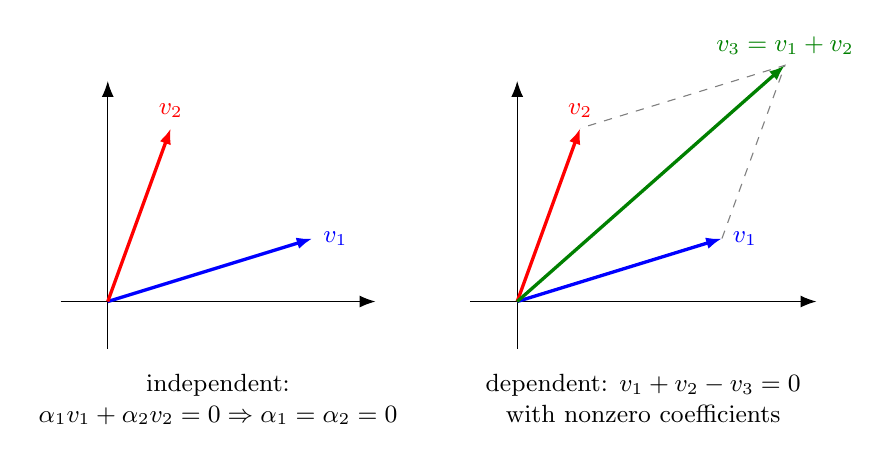
\begin{tikzpicture}[every node/.style={font=\small}, >={Latex[length=2mm]}]
	\draw[->] (-0.6,0) -- (3.4,0);
	\draw[->] (0,-0.6) -- (0,2.8);
	\draw[->, blue, very thick] (0,0) -- (2.6,0.8) node[right] {$v_1$};
	\draw[->, red, very thick] (0,0) -- (0.8,2.2) node[above] {$v_2$};
	\node[anchor=north, align=flush center, text width=4.6cm] at (1.4,-0.8) {independent: $\alpha_1v_1+\alpha_2v_2=0\Rightarrow\alpha_1=\alpha_2=0$};
	\begin{scope}[xshift=5.2cm]
		\draw[->] (-0.6,0) -- (3.8,0);
		\draw[->] (0,-0.6) -- (0,2.8);
		\draw[->, blue, very thick] (0,0) -- (2.6,0.8) node[right] {$v_1$};
		\draw[->, red, very thick] (0,0) -- (0.8,2.2) node[above] {$v_2$};
		\draw[->, green!50!black, very thick] (0,0) -- (3.4,3.0) node[above] {$v_3=v_1+v_2$};
		\draw[dashed, gray] (2.6,0.8) -- (3.4,3.0) -- (0.8,2.2);
		\node[anchor=north, align=flush center, text width=4.6cm] at (1.6,-0.8) {dependent: $v_1+v_2-v_3=0$ with nonzero coefficients};
	\end{scope}
\end{tikzpicture}
\end{document}
